\subsection{Centered Parabola-shaped Branches}
\label{sec:setup.quad.even}

\hl{
	This section examines the piecewise-quadratic model with the centered parabola-shaped branches, see the functions in \Cref{fig:setup.quad.even.cobwebs}.
	To center the parabola-shaped branches, the parameter values $a_L = a_R = 6$, $b_L = -\frac{3}{2}$, and $b_R = -\frac{9}{2}$ are chosen and only the parameters $c_L$ and $c_R$ are varied.
	Both varied parameters are in the ranges $[0.25, 0.6]$.
}

This emulates the effect that $\chi_0$ has on the branches $F_\A$ and $F_\C$.
Increasing $c_L$ increases the values of the branches $f_\A$ and $f_\C$.
\hl{
	The effects of $E_0$ on branches $F_\B$ and $F_\D$ are lowering the values of the function on the left sides of the branches, moving the local minima of the branches to the left, and reducing the value of the function at the minima.
}
Decreasing $c_R$ does not have the same effects \hl{on the branches $f_\B$ and $f_\D$} but rather lowers the \hl{values of the function for} the whole branches.
\Cref{fig:setup.quad.even.period.full} \hl{shows 2D scans of the periods associated with parameter regions in this model}.

\begin{figure}
	\centering
	\begin{subfigure}{0.4\textwidth}
		\centering
		\includegraphics[width=\textwidth]{21_Quadratic_mod1/2D_Period_Zoomed1/result.png}
		\caption{Full}
		\label{fig:setup.quad.even.period.full}
	\end{subfigure}
	\begin{subfigure}{0.4\textwidth}
		\centering
		\includegraphics[width=\textwidth]{21_Quadratic_mod1/2D_Period_Zoomed2/result.png}
		\caption{Zoomed}
		\label{fig:setup.quad.even.period.zoomed}
	\end{subfigure}
	\caption[2D scans showing periods of the even piecewise quadratic model]{
		2D scans showing the periods of the piecewise-quadratic model with fixed parameters $a_L = a_R = 6$, $b_L = -\frac{3}{2}$, and $b_R = -\frac{9}{2}$.
		(a) shows the full structure with parameters $c_L$ and $c_R$ varied in the range $[0.25, 0.6]$ each.
		The red rectangle marks the parameter range that \hl{is shown magnified in} (b).
		The marked points in (b) are the parameter values for the \hl{cobweb diagrams} in \Cref{fig:setup.quad.even.cobwebs}
	}
\end{figure}

\begin{figure}
	\centering
	\begin{subfigure}{0.3\textwidth}
		\centering
		\includegraphics[width=\textwidth]{21_Quadratic_mod1/Cobweb_A/result.png}
		\caption{At point $A$}
		\label{fig:setup.quad.even.cobweb.A}
	\end{subfigure}
	\begin{subfigure}{0.3\textwidth}
		\centering
		\includegraphics[width=\textwidth]{21_Quadratic_mod1/Cobweb_B/Manual/result.png}
		\caption{At point $B$}
		\label{fig:setup.quad.even.cobweb.B}
	\end{subfigure}
	\begin{subfigure}{0.3\textwidth}
		\centering
		\includegraphics[width=\textwidth]{21_Quadratic_mod1/Cobweb_C/result.png}
		\caption{At point $C$}
		\label{fig:setup.quad.even.cobweb.C}
	\end{subfigure}
	\caption[Cobwebs of the even quadratic model]{
		Cobweb diagrams at three parameter values of $c_L$ and $c_R$ in the piecewise quadratic model with fixed parameters $a_L = a_R = 6$, $b_L = -\frac{3}{2}$, and $b_R = -\frac{9}{2}$.
		The parameter values are marked in \Cref{fig:setup.quad.even.period.zoomed}.
		(a) shows the cycle $\Cycle{\A^3\B\C^3\D}$ at point $A$ \hl{where $c_L = 0.2925$ and $c_R = 0.41$},
		(b) shows the two coexisting cycles $\Cycle{\A^3\B\C^3\D}$ (green) and $\Cycle{\A^2\B\C^2\D}$ (red) at the point $B$ \hl{where $c_L = 0.2975$ and $c_R = 0.425$},
		and (c) shows the cycle $\Cycle{\A^2\B\C^2\D}$ at the point $C$ where \hl{$c_L = 0.3025$ and $c_R = 0.44$}.
	}
	\label{fig:setup.quad.even.cobwebs}
\end{figure}

A phenomenon like in the original model \hl{can} not be found here.
But something very similar happens at the border of these wings.
\Cref{fig:setup.quad.even.cobwebs} shows the cobwebs at the points marked in \Cref{fig:setup.quad.even.period.zoomed}.
At point $A$, there is one stable cycle with period $8$.
This cycle is depicted in \Cref{fig:setup.quad.even.cobweb.A} and its symbolic sequence is $\A^3B\C^3\D$.
Point $B$ is in a parameter region, where 2 stable cycles coexist.
\hl{One can not} see this in the 2D scans in \Cref{fig:setup.quad.even.period.full}, since it only ever picks up on one cycle.
\Cref{fig:setup.quad.even.cobweb.B} shows the coexisting cycles at this border.
\hl{
	The symbolic sequences of the two coexisting cycles are $\A^3B\C^3\D$ and $\A^2\B\C^2\D$.
}
In contrast to the original model, the cycle that existed before in \Cref{fig:setup.quad.even.cobweb.A} \hl{with the symbolic sequence $\A^3B\C^3\D$} still exists alongside the new cycle with \hl{the symbolic sequence $\A^2\B\C^2\D$}.
\hl{
	At point $C$, there is again only one stable cycle.
	It has the period $6$ and the symbolic sequence $\A^2\B\C^2\D$.
	Therefore, this is the cycle that coexisted with the cycle with the symbolic sequence $\A^3B\C^3\D$ at point $C$.
}

This is different from the dynamics in the original model in two ways.
First, the cycles before and after the \hl{parameter region} of coexistence have different periods.
And second, the cycles existing outside the \hl{parameter region} of coexistence still exist inside the \hl{parameter region} of coexistence.
In the original model, the cycles existing outside the \hl{parameter region} of coexistence would disappear at the boundaries and new cycles would emerge inside this \hl{parameter region}.
Here, \hl{one} simply observes two overlapping parameter regions which is something different from the original model.
